\documentclass{article}
\usepackage{amsfonts, amsthm, amsmath, amssymb, mathtools, ulem, mathrsfs, physics, esint, siunitx, tikz-cd}
\usepackage{pdfpages, fullpage, color, microtype, cancel, textcomp, markdown, hyperref, graphicx}
\usepackage{enumitem}
\graphicspath{{./images/}}
\usepackage[english]{babel}
\usepackage[autostyle, english=american]{csquotes}
\MakeOuterQuote{"}
\usepackage{xparse}
\usepackage{tikz}
\usepackage{nicematrix}

% fonts
\def\mbb#1{\mathbb{#1}}
\def\mfk#1{\mathfrak{#1}}
\def\mbf#1{\mathbf{#1}}
\def\tbf#1{\textbf{#1}}

% common bold letters
\def\bP{\mbb{P}}
\def\bC{\mbb{C}}
\def\bH{\mbb{H}}
\def\bI{\mbb{I}}
\def\bR{\mbb{R}}
\def\bQ{\mbb{Q}}
\def\bZ{\mbb{Z}}
\def\bN{\mbb{N}}

% brackets
\newcommand{\br}[1]{\left(#1\right)}
\newcommand{\sbr}[1]{\left[#1\right]}
\newcommand{\brc}[1]{\left\{#1\right\}}
\newcommand{\lbr}[1]{\left\langle#1\right\rangle}

% matrices
\newcommand{\m}[2][b]{\begin{#1matrix}#2\end{#1matrix}}
\newcommand{\arr}[3][\sbr]{#1{\begin{array}{#2}#3\end{array}}}
\DeclareMathOperator{\Span}{span}
\DeclareMathOperator{\diag}{diag}
\DeclareMathOperator{\Null}{null}
\DeclareMathOperator{\range}{range}

% greek
\newcommand{\e}{\epsilon}
\newcommand{\p}{\varphi}
\renewcommand{\t}{\sim}
\renewcommand{\L}{\Lambda}
\renewcommand{\l}{\lambda}
\newcommand{\s}{\sigma}
\renewcommand{\S}{\Sigma}

% misc
\NewDocumentCommand{\app}{O{x} O{\infty}}{\xrightarrow{#1\to#2}}
\newcommand{\sse}{\subseteq}
\renewcommand{\ss}{\subset}
\newcommand{\vn}{\varnothing}
\newcommand{\inv}{^{-1}}
\newcommand{\imp}{\implies}
\newcommand{\impleft}{\reflectbox{$\implies$}}
\renewcommand{\ip}[2]{\lbr{#1,#2}}
\renewcommand{\bar}{\overline}
\DeclareMathOperator{\cis}{cis}
\DeclareMathOperator{\Arg}{Arg}
\renewcommand{\d}{\partial}
\newcommand{\pf}{\tbf{Proof. }}
\DeclareMathOperator{\sign}{sign}
\renewcommand{\u}{\tilde{u}}
\DeclareMathOperator{\House}{House}

% title
\title{Scientific Computing HW 3}
\author{Ryan Chen}
%\date{\today}
\setlength{\parindent}{0pt}


\begin{document}
	
\maketitle



\begin{enumerate}
	
	
	
	\item 
	
	\begin{enumerate}
		
		
		
		\item Compute
		\begin{align*}
			P^T &= I^T - 2(uu^T)^T \\
			&= I - 2(u^T)^Tu^T \\
			&= I - 2uu^T \\
			&= P
		\end{align*}
		Using $u^Tu=1$,
		\begin{align*}
			P^2 &= (I - 2uu^T)(I - 2uu^T) \\
			&= I^2 - 2Iuu^T - 2uu^TI + 4uu^Tuu^T \\
			&= I - 4uu^T + 4uu^T \\
			&= I
		\end{align*}
		
		
		
		\item Using $\sign(a)^2=1$ and $\sign(a)a=|a|$, compute
		\[\u^Tx = \norm{x}^2 + \sign(x_1)x_1\norm{x} = \norm{x}^2 + |x_1|\norm{x}\]
		\[\u^T\u = \norm{x}^2 + \sign(x_1)^2\norm{x}^2 + 2\sign(x_1)x_1\norm{x} = 2\norm{x}^2 + 2|x_1|\norm{x}\]
		Then compute
		\begin{align*}
			Px &= x - 2\frac{\u^Tx}{\u^T\u}\u \\
			&= x - \u \\
			&= -\sign(x_1)\norm{x}e_1
		\end{align*}
		
		
		
		\item For convenience, write matrix entries as superscripts, reserving subscripts for the iteration described in the problem. We will prove using finite induction that for $1\le j\le n$, the first $j$ diagonal entries of $A_{j}$ are
		\[-\sign(A_0^{11})\norm{A_0(1:m,1)}, \dots, -\sign(A_{j-1}^{jj})\norm{A_{j-1}(j:m,j)}\]
		and that the entries below the first $j$ diagonal entries are zero.
		
		The case $j=1$ is proven by $\House(A_0(1:m,1))A_0(1:m,1)=-\sign(A_0^{11})\norm{A_0(1:m,1)}e_1$, which is the first column of $A_1=P_1A_0$.
		
		Assume the claim is true for $j$. Then (use $\t$ to denote possibly nonzero entries)
		\[A_j =
		\arr{ccc|c}{
		-\sign(A_0^{11})\norm{A_0(1:m,1)} & & \t & \\
		& \ddots & & \t \\
		& & -\sign(A_{j-1}^{jj})\norm{A_{j-1}(j:m,j)} & \\
		\hline
		& 0_{(m-j)\times j} & & \t
		}\]
		From the algorithm,
		\[P_{j+1} =
		\arr{c|c}{
		I_{j\times j} & 0_{j\times(m-j)} \\
		\hline
		0_{(m-j)\times j} & \House(A_j(j+1:m,j+1))
		}\]
		Then, by the fact $\House(A_j(j+1:m,j+1))A_j(j+1:m,j+1)=-\sign(A_j^{j+1,j+1})\norm{A_j(j+1:m,j+1)}e_1$,
		\[A_{j+1} = P_{j+1}A_j =
		\arr{ccc|c}{
			-\sign(A_0^{11})\norm{A_0(1:m,1)} & & \t & \\
			& \ddots & & \t \\
			& & -\sign(A_{j}^{j+1,j+1})\norm{A_{j}(j+1:m,j+1)} & \\
			\hline
			& 0_{(m-j-1)\times(j+1)} & & \t
		}\]
		This closes the induction. Having proven the claim, setting $j=n$ gives
		\[A_n =
		\arr{ccc}{
			-\sign(A_0^{11})\norm{A_0(1:m,1)} & & \t \\
			& \ddots & \\
			& & -\sign(A_{n-1}^{nn})\norm{A_{n-1}(n:m,n)} \\
			\hline
			& 0_{(m-n)\times n} &
		}\]
		
		To guarantee that $A_n$ has positive diagonal entries, note that
		\[-\sign(A_{j-1}^{jj})\norm{A_{j-1}(j:m,j)} > 0
		\iff -\sign(A_{j-1}^{jj}) > 0
		\iff A_{j-1}^{jj} < 0\]
		If $A_{j-1}^{jj}>0$, change its sign before constructing $P_j$.
		
		
		
		\item From the iteration,
		\[A_n = P_nP_{n-1}\dots P_1A\]
		From $P_j^2=I$, we have $P_j\inv=P_j$, hence
		\[(P_nP_{n-1}\dots P_1)\inv = P_1\inv P_2\inv\dots P_n\inv = P_1P_2\dots P_n\]
		Which in turn gives a QR decomposition of $A$.
		\[A = \underbrace{P_1\dots P_n}_{=:Q}\underbrace{A_n}_{=:R}\]
		
		 
	\end{enumerate}

	
	
	\pagebreak
	
	

	\item
	
	\begin{enumerate}
		
		
		
		\item From the eigendecomposition $A=U\L U^T$, we see $U$ is orthogonal, so its columns $u_1,\dots,u_n$ form an orthonormal basis of $\bR^n$, and $A$ has eigenpairs $(\l_i,u_i)$. Define
		\[\S := \diag(\s_1,\dots,\s_n),
		\quad \s_i := |\l_i|\]
		\[V := \m{v_1 & \dots & v_n},
		\quad v_i := s_iu_i,
		\quad s_i := \sign(\l_i)\]
		Then we have
		\[V = U\diag(s_1,\dots,s_n),
		\quad V^T = \diag(s_1,\dots,s_n)U^T,
		\quad \diag(s_1,\dots,s_n)^2 = I_{n\times n}\]
		The last equation comes from the fact that $\sign(x)^2=1$. Hence
		\begin{align*}
			V^TV &= \diag(s_1,\dots,s_n)U^TU\diag(s_1,\dots,s_n) \\
			&= \diag(s_1,\dots,s_n)^2 & \text{$U$ is orthogonal} \\
			&= I_{n\times n} & \diag(s_1,\dots,s_n)^2 = I_{n\times n}
		\end{align*}
		and
		\begin{align*}
			VV^T &= U\diag(s_1,\dots,s_n)^2U^T \\
			&= UU^T & \diag(s_1,\dots,s_n)^2 = I_{n\times n} \\
			&= I_{n\times n} & \text{$U$ is orthogonal}
		\end{align*}
		Thus $V$ is orthogonal.
		
		Lastly, we check that $A=U\S V^T$ by showing that the action of both sides agrees on the basis $u_1,\dots,u_n$ of $\bR^n$, i.e. $Au_i=U\S V^Tu_i$ for $1\le i\le n$.
		\begin{align*}
			U\S V^Tu_i &= U\S(s_ie_i) & \text{the $u_i$'s are orthonormal} \\
			&= U(s_i|\l_i|e_i) \\
			&= U(\l_ie_i) & \sign(x)|x| = x \\
			&= \l_iu_i \\
			&= Au_i & \text{$(\l_i,u_i)$ is an eigenpair of $A$}
		\end{align*}
		
		
		
		\item Using the SVD $A=U\S V^T$,
		\begin{align*}
			A^TA &= V\S U^TU\S V^T \\
			&= V\S^2V^T & U^TU = I_{n\times n} \\
			&= V\diag(\s_1^2,\dots,\s_n^2)V^T
		\end{align*}
		This is an eigendecomposition of $A^TA$ with eigenpairs $(\s_i^2,v_i)$.
		
		
		
		\item Via the "basis extension theorem" and the Gram--Schmidt process, we can extend the linearly independent orthonormal set $u_1,\dots,u_n$ to an orthonormal basis $u_1,\dots,u_n,u_{n+1},\dots,u_m$ of $\bR^m$. Since $AA^T$ is $m\times m$, it requires an $m\times m$ eigendecomposition.
		\begin{align*}
			AA^T &= U\S V^TV\S U^T \\
			&= U\S^2U^T \\
			&= \arr{c|c|c|c}{U & u_{n+1} & \dots & u_m}
				\arr{c|c}{
				\S^2 & 0_{n\times(m-n)} \\
				\hline
				0_{(m-n)\times n} & 0_{(m-n)\times(m-n)}
				}
				\arr{c}{U^T \\ \hline u_{n+1}^T \\ \hline \vdots \\ \hline u_m^T}			
		\end{align*}
		This is an eigendecomposition of $AA^T$ with eigenpairs $(\s_i^2,u_i)$ for $1\le i\le n$ and $(0,u_i)$ for $n+1\le i\le m$.
		
		
		
		\item From $A$ being full rank, the least squares solution to $Ax=b$ is $x^*=(A^TA)\inv A^Tb$. From the SVD $A=U\S V^T$ and the fact $A$ is full rank (so that $A^TA$ and $\S$ are nonsingular),
		\[A^TA = V\S^2V^T
		\imp (A^TA)\inv = V(\S\inv)^2 V^T\]
		Hence
		\begin{align*}
			x^* &= (A^TA)\inv A^Tb \\
			&= V(\S\inv)^2 V^TV\S U^Tb \\
			&= V(\S\inv)^2SU^Tb \\
			&= V\S\inv U^Tb
		\end{align*}
		
		
		
		\item We use the fact that $\norm{A}_2$ equals the largest singular value of $A$. From the SVD $A=U\S V^T$ and the fact $A$ is nonsingular ($\S$ is nonsingular), we have $A\inv=V\S\inv U^T$, an SVD of $A\inv$. Assume the singular values of $A$ are arranged in decreasing order, $\s_1\ge\dots\ge\s_n>0$. Then $\S\inv$ gives the singular values of $A\inv$, which arranged in decreasing order are $\frac{1}{\s_n}\ge\dots\ge\frac{1}{\s_1}$. Thus $\norm{A\inv}_2=\frac{1}{\s_n}$.
		
		
		
		\item Throughout we use the fact that $Av_i=\s_iu_i$ for $1\le i\le n$, and that for vectors $w_1,\dots,w_k$, $\Span(w_1,\dots,w_k)$ is the smallest subspace containing $w_1,\dots,w_k$.
		
		We first show that $\Null(A)=\Span(v_{r+1},\dots,v_n)$.
		\begin{itemize}
			\item Let $x\in\Null(A)$. Using the basis $v_1,\dots,v_n$, write
			\[x=\sum_{i=1}^nc_iv_i\]
			for some $c_1,\dots,c_n\in\bR$. This, along with $Ax=0$ and $Av_i=\s_iu_i$, gives
			\[\sum_{i=1}^r c_i\s_iu_i=0\]
			Since the $u_i$'s are linearly independent, $c_i\s_i=0$, hence $c_i=0$, for $1\le i\le r$. Thus
			\[x=\sum_{i=r+1}^n c_iv_i\in\Span(v_{r+1},\dots,v_n)\] 
			We conclude $\Null(A)\ss\Span(v_{r+1},\dots,v_n)$.
			\item For $r+1\le i\le n$, we have $Av_i=\s_iu_i=0$, so $v_i\in\Null(A)$. Then $\Null(A)$ is a subspace of $\bR^n$ containing $v_{r+1},\dots,v_n$, hence $\Span(v_{r+1},\dots,v_n)\ss\Null(A)$.
		\end{itemize}
	
		Then we show that $\range(A)=\Span(u_1,\dots,u_r)$.
		\begin{itemize}
			\item Let $y\in\range(A)$. Then $y=Ax$ for some $x\in\bR^n$. Using the basis $v_1,\dots,v_n$, write
			\[x=\sum_{i=1}^nc_iv_i\]
			for some $c_1,\dots,c_n\in\bR$. This, along with $Av_i=\s_iu_i$, gives
			\[y=Ax=\sum_{i=1}^r c_i\s_iu_i\in\Span(u_1,\dots,u_r)\]
			Thus $\range(A)\ss\Span(u_1,\dots,u_r)$.
			\item For $1\le i\le r$, using the fact $Av_i=\s_iu_i$, we have $u_i=A\br{\frac{1}{\s_i}v_i}\in\range(A)$. Then $\range(A)$ is a subspace of $\bR^m$ containing $u_1,\dots,u_r$, hence $\Span(u_1,\dots,u_r)\ss\range(A)$.
		\end{itemize}
	
		From $\range(A)=\Span(u_1,\dots,u_r)$ and the $u_i$'s being linearly independent, we see that $u_1,\dots,u_r$ form a basis of $\range(A)$, hence $\rank(A)=r$.
		
		
		
		
	\end{enumerate}

	
	
	\pagebreak
	
	

	\item The claim is that (here we omit the subscript for the 2--norm)
	\[\min_{Ax=b}\norm{x}=\norm{x^*}\]
	First we see that $x^*$ solves $Ax=b$.
	\[Ax^* = AA^T(AA^T)\inv b = b\]
	Now let $x$ solve $Ax=b$. Then
	\[Ax = Ax^*
	\imp A(x-x^*) = 0\]
	From this,
	\[(x-x^*)^Tx^* = (x-x^*)^TA^T(AA^T)\inv b
	= (A(x-x^*))^T(AA^T)\inv b
	= 0\]
	In turn, we get
	\[\norm{x}^2 = \norm{(x-x^*)+x^*}^2
	= \norm{x-x^*}^2 + \norm{x^*}^2 + 2(x-x^*)^Tx^*
	= \norm{x-x^*}^2 + \norm{x^*}^2
	\ge \norm{x^*}^2\]
	Hence $Ax^*=b$, with $\norm{x}\ge\norm{x^*}$ whenever $Ax=b$. This establishes the claim.
	
	
	
	\pagebreak
	
	
	
	\item
	
	\begin{enumerate}
		
		
		
		
		\item From the Schur decomposition $A=QTQ^*$, we have $AQ=QT$. If $(\l,v)$ is an eigenpair of $T$, write $Tv=\l v$, so that $AQv=QTv=\l Qv$, hence $(\l,Qv)$ is an eigenpair of $A$.
		
		
		
		\item Since $T$ is upper triangular, its eigenvalues are the diagonal entries $\l_1,\l_2,\l_3$.
		
		Moreover, $Te_1=\l_1e_1$, confirming $(\l_1,v_1)$ as an eigenpair with $v_1=e_1$.
		
		Seeking an eigenpair of the form $(\l_2,v_2)$ with $v_2=[a,1,0]^T$, compute
		\[Tv_2 = \m{\l_1a+t_{12} \\ \l_2 \\ 0},
		\quad \l_2v_2 = \m{\l_2a \\ \l_2 \\ 0}\]
		Equating the first components,
		\[\l_1a + t_{12} = \l_2a
		\imp (\l_2-\l_1) = t_{12}
		\imp a = \frac{t_{12}}{\l_2-\l_1}\]
		
		Seeking an eigenpair of the form $(\l_3,v_2)$ with $v_3=[b,c,1]^T$, compute
		\[Tv_3 = \m{\l_1b + t_{12}c + t_{13} \\ \l_2c + t_{23} \\ \l_3},
		\quad \l_3v_3 = \m{\l_3b \\ \l_3c \\ \l_3}\]
		Equating the second components,
		\[\l_2c + t_{23} = \l_3c
		\imp (\l_3-\l_2)c = t_{23}
		\imp c = \frac{t_{23}}{\l_3-\l_2}\]
		Equating the first components,
		\[\l_1b + t_{12}c + t_{13} = \l_3b
		\imp (\l_3-\l_1)b = t_{12}c + t_{13}
		\imp b = \frac{t_{12}c}{\l_3-\l_1} + \frac{t_{13}}{\l_3-\l_1}\]
		Using the formula for $c$,
		\[b = \frac{t_{12}t_{23}}{(\l_3-\l_1)(\l_3-\l_2)} + \frac{t_{13}}{\l_3-\l_1}\]
		
		
		
		\item By parts (a) and (b), eigenvectors of $A$ are
		\[Qv_1 = Qe_1 = q_1\]
		\[Qv_2 = aq_1 + q_2\]
		\[Qv_3 = bq_1 + cq_2 + q_3\]
		where
		\[a = \frac{t_{12}}{\l_2-\l_1},
		\quad b = \frac{t_{12}t_{23}}{(\l_3-\l_1)(\l_3-\l_2)} + \frac{t_{13}}{\l_3-\l_1},
		\quad c = \frac{t_{23}}{\l_3-\l_2}\]
		
		
		
	\end{enumerate}
	
	
	
	\pagebreak
	
	
	
	\item Code: \url{https://github.com/RokettoJanpu/scientific-computing-1-redux/blob/main/hw3.ipynb}
	
	\begin{enumerate}
		
		
		
		\item 
		
		\begin{center}
			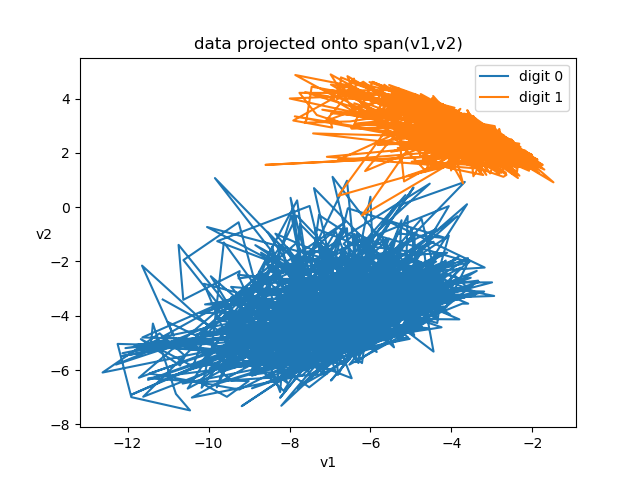
\includegraphics[scale=.7]{hw3 projection}
		\end{center}
		Indeed, 0s and 1s cluster in this space.
		
		
		
		\item
		
		\begin{center}
			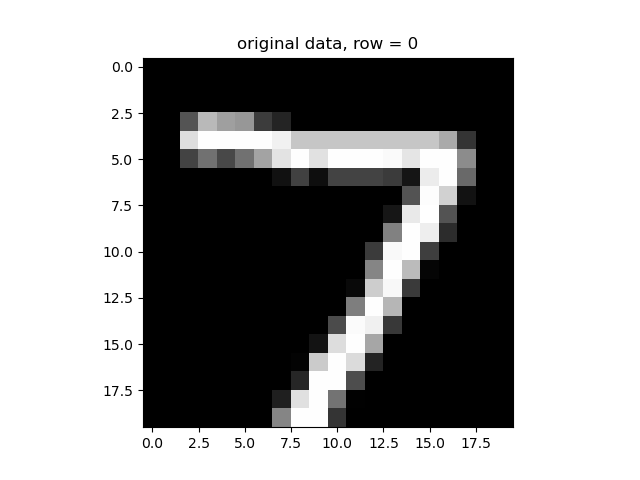
\includegraphics[scale=.4]{hw3 orig, row = 0}
			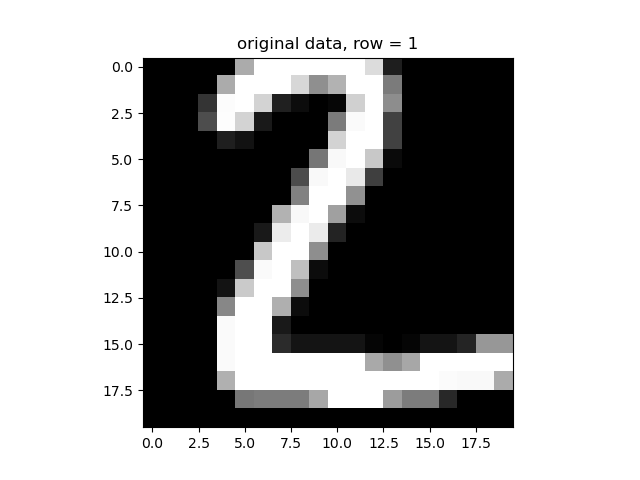
\includegraphics[scale=.4]{hw3 orig, row = 1}
			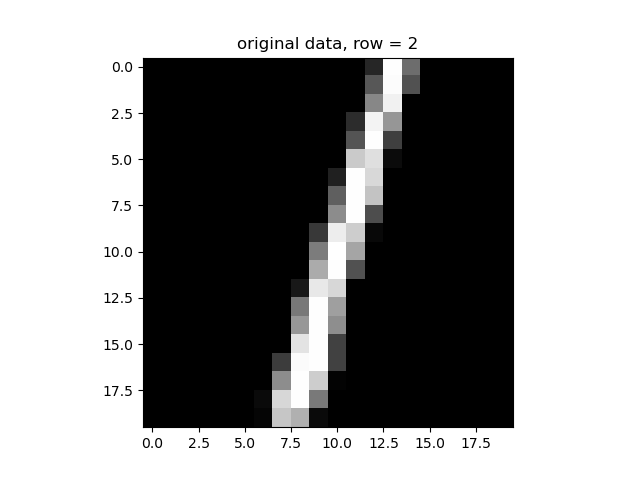
\includegraphics[scale=.4]{hw3 orig, row = 2}
			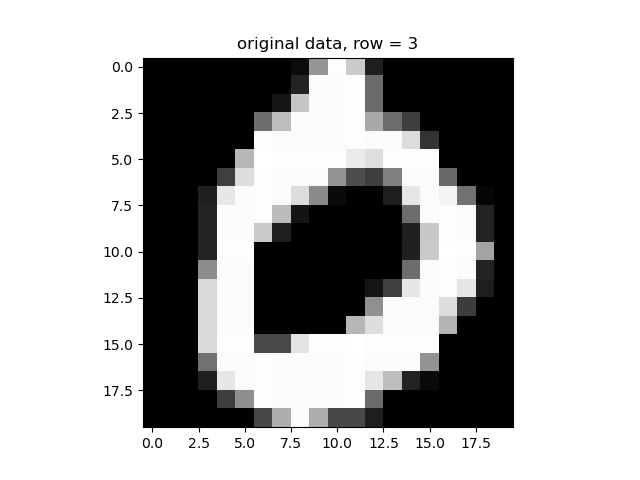
\includegraphics[scale=.4]{hw3 orig, row = 3}
			
			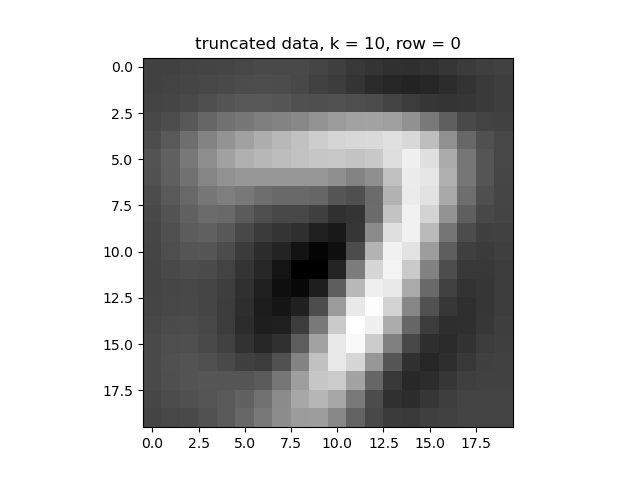
\includegraphics[scale=.4]{hw3 trunc, k = 10, row = 0}
			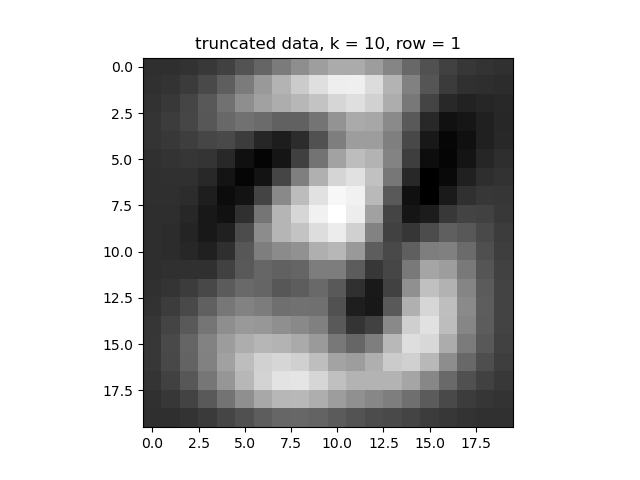
\includegraphics[scale=.4]{hw3 trunc, k = 10, row = 1}
			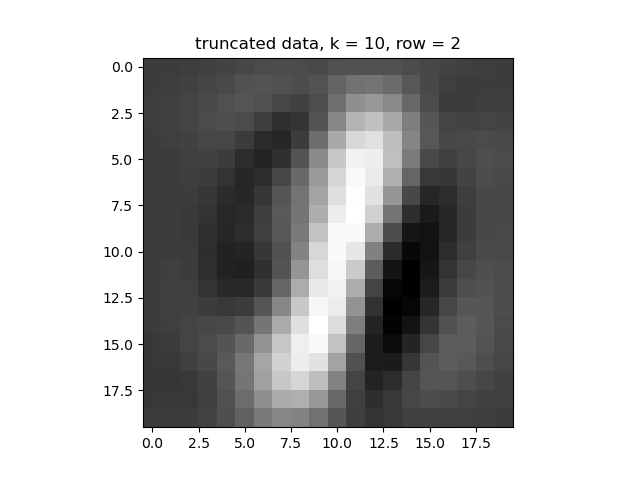
\includegraphics[scale=.4]{hw3 trunc, k = 10, row = 2}
			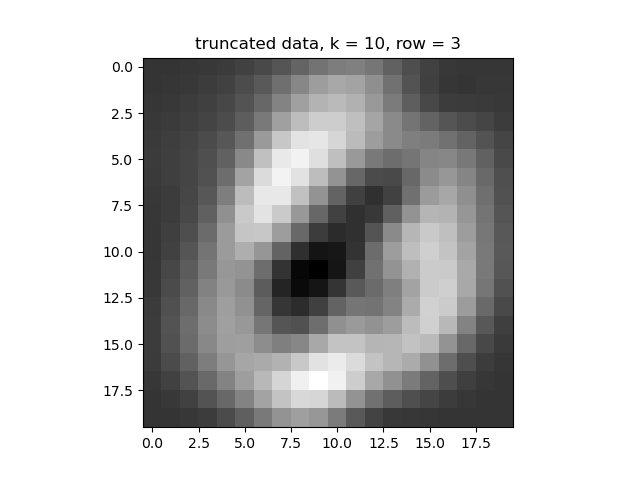
\includegraphics[scale=.4]{hw3 trunc, k = 10, row = 3}
			
			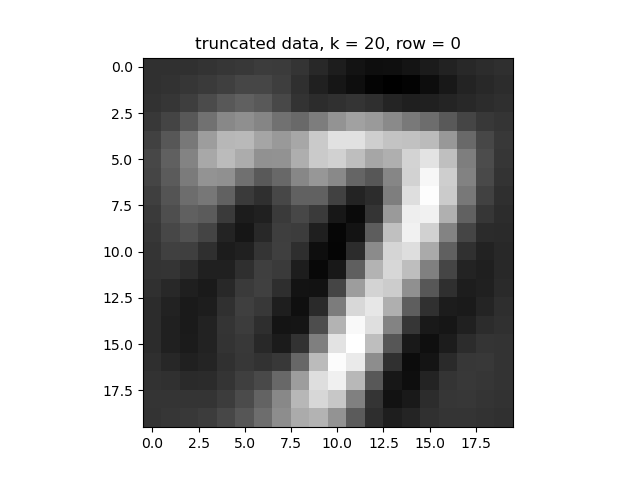
\includegraphics[scale=.4]{hw3 trunc, k = 20, row = 0}
			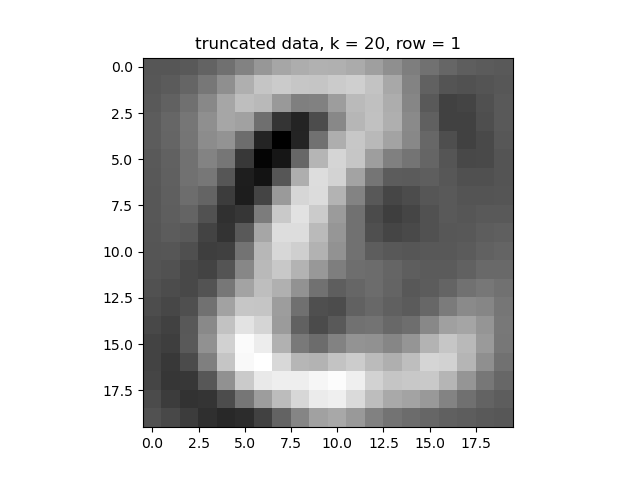
\includegraphics[scale=.4]{hw3 trunc, k = 20, row = 1}
			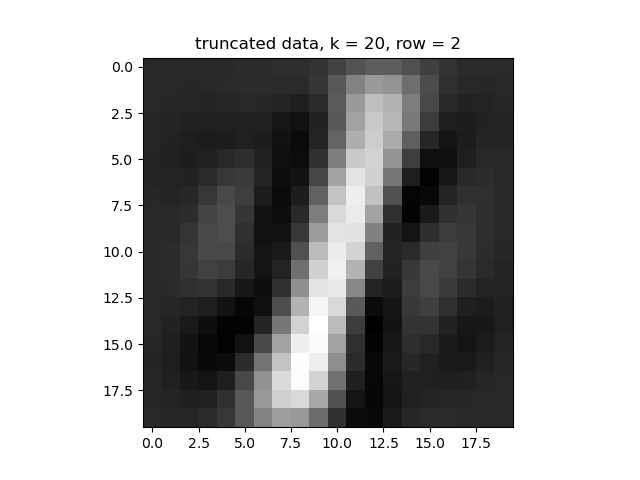
\includegraphics[scale=.4]{hw3 trunc, k = 20, row = 2}
			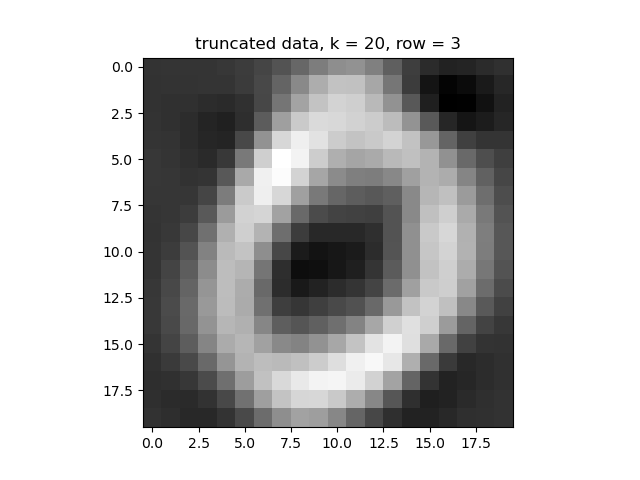
\includegraphics[scale=.4]{hw3 trunc, k = 20, row = 3}
			
			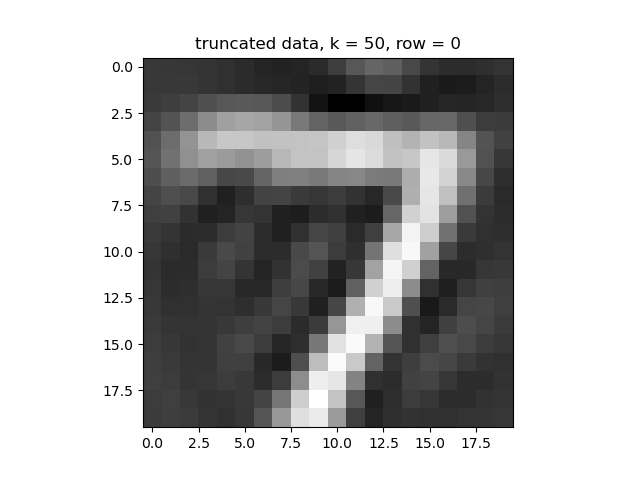
\includegraphics[scale=.4]{hw3 trunc, k = 50, row = 0}
			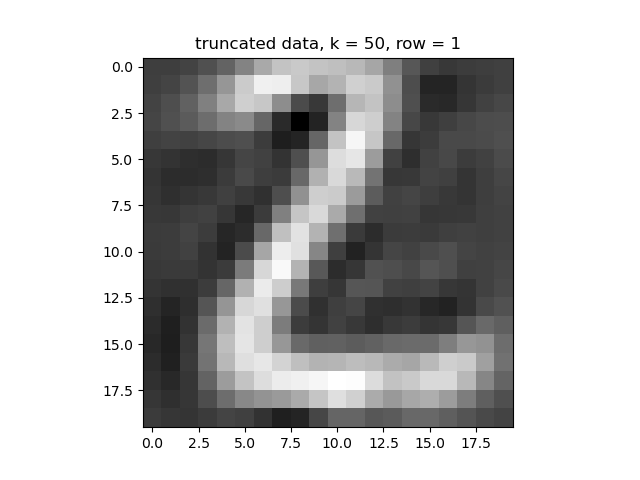
\includegraphics[scale=.4]{hw3 trunc, k = 50, row = 1}
			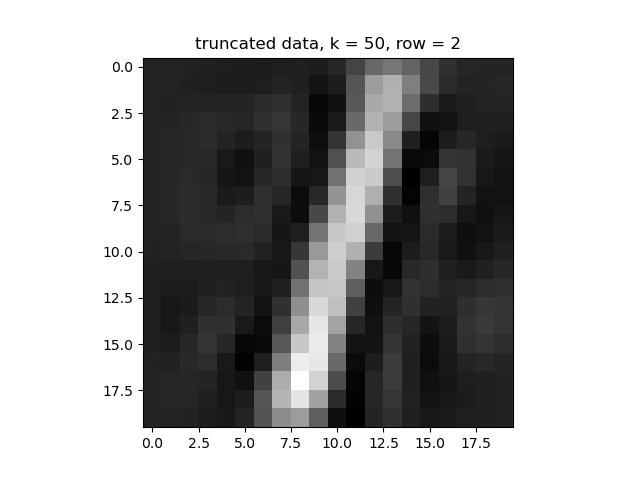
\includegraphics[scale=.4]{hw3 trunc, k = 50, row = 2}
			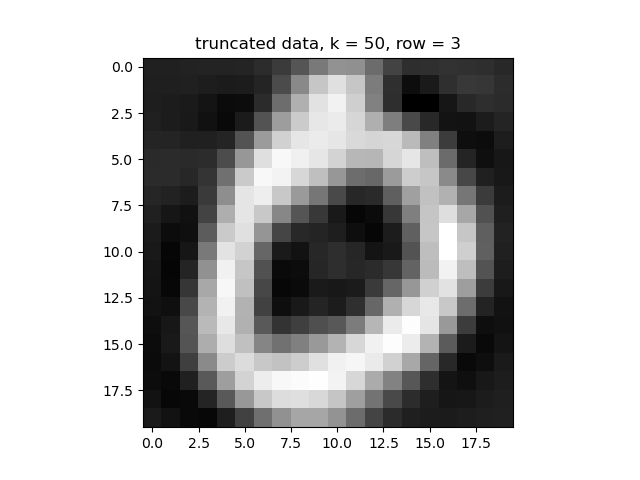
\includegraphics[scale=.4]{hw3 trunc, k = 50, row = 3}
		\end{center}
		
		
		
	\end{enumerate}
	
	
	
\end{enumerate}
	
	
\end{document}